%
% A header that lets you compile a chapter by itself, or inside a larger document.
% Adapted from stackoverflow.com/questions/3655454/conditional-import-in-latex
%
%
%Use \inbpdocument and \outbpdocument in your individual files, in place of \begin{document} and \end{document}. In your main file, put in a \def \ismaindoc {} before including or importing anything.
%
% David Duvenaud
% June 2011
% 
% ======================================
%
%


\ifx\ismaindoc\undefined
	\newcommand{\inbpdocument}{
		\def \ismaindoc {}
		% Use this header if we are compiling by ourselves.
		\documentclass[a4paper,11pt,authoryear,index]{common/PhDThesisPSnPDF}
		
%\usepackage{draftwatermark}
%\SetWatermarkLightness{0.95}

% ******************************************************************************
% ****************************** Custom Margin *********************************

% Add `custommargin' in the document class options to use this section
% Set {innerside margin / outerside margin / topmargin / bottom margin}  and
% other page dimensions

\ifsetMargin
\else
    \RequirePackage[left=37mm,right=30mm,top=35mm,bottom=30mm]{geometry}
    \setFancyHdr % To apply fancy header after geometry package is loaded
\fi


%\chead{Unfinished draft}
%\cfoot{\texttt{Unfinished draft - compiled on \today{} at \currenttime}}

% *****************************************************************************
% ******************* Fonts (like different typewriter fonts etc.)*************

% Add `customfont' in the document class option to use this section

\ifsetFont
\else
    % Set your custom font here and use `customfont' in options. Leave empty to
    % load computer modern font (default LaTeX font).  

    \RequirePackage{libertine} 
\fi

% *****************************************************************************
% *************************** Bibliography  and References ********************

%\usepackage{cleveref} %Referencing without need to explicitly state fig /table

% Add `custombib' in the document class option to use this section
\ifsetBib % True, Bibliography option is chosen in class options
\else % If custom bibliography style chosen then load bibstyle here

   \RequirePackage[square, sort, numbers, authoryear]{natbib} % CustomBib

% If you would like to use biblatex for your reference management, as opposed to the default `natbibpackage` pass the option `custombib` in the document class. Comment out the previous line to make sure you don't load the natbib package. Uncomment the following lines and specify the location of references.bib file

% \RequirePackage[backend=biber, style=numeric-comp, citestyle=numeric, sorting=nty, natbib=true]{biblatex}
% \bibliography{References/references} %Location of references.bib only for biblatex

\fi


% changes the default name `Bibliography` -> `References'
\renewcommand{\bibname}{References}


% *****************************************************************************
% *************** Changing the Visual Style of Chapter Headings ***************
% Uncomment the section below. Requires titlesec package.

%\RequirePackage{titlesec}
%\newcommand{\PreContentTitleFormat}{\titleformat{\chapter}[display]{\scshape\Large}
%{\Large\filleft{\chaptertitlename} \Huge\thechapter}
%{1ex}{}
%[\vspace{1ex}\titlerule]}
%\newcommand{\ContentTitleFormat}{\titleformat{\chapter}[display]{\scshape\huge}
%{\Large\filleft{\chaptertitlename} \Huge\thechapter}{1ex}
%{\titlerule\vspace{1ex}\filright}
%[\vspace{1ex}\titlerule]}
%\newcommand{\PostContentTitleFormat}{\PreContentTitleFormat}
%\PreContentTitleFormat


% *****************************************************************************
% **************************** Custom Packages ********************************
% *****************************************************************************


% ************************* Algorithms and Pseudocode **************************

%\usepackage{algpseudocode} 


% ********************Captions and Hyperreferencing / URL **********************

% Captions: This makes captions of figures use a boldfaced small font. 
%\RequirePackage[small,bf]{caption}

\RequirePackage[labelsep=space,tableposition=top]{caption} 
%\renewcommand{\figurename}{Figure} %to support older versions of captions.sty
\captionsetup{labelsep = colon,belowskip=12pt,aboveskip=4pt}

% ************************ Formatting / Footnote *******************************

%\usepackage[perpage]{footmisc} %Range of footnote options 


% ****************************** Line Numbers **********************************

%\RequirePackage{lineno}
%\linenumbers

% ************************** Graphics and figures *****************************

%\usepackage{rotating}
%\usepackage{wrapfig}
%\usepackage{float}
\usepackage{subfig} %note: subfig must be included after the `caption` package. 


% ********************************* Table **************************************

%\usepackage{longtable}
%\usepackage{multicol}
%\usepackage{multirow}
%\usepackage{tabularx}


% ***************************** Math and SI Units ******************************

\usepackage{amsfonts}
\usepackage{amsmath}
\usepackage{amssymb}
%\usepackage{siunitx} % use this package module for SI units


% ******************************************************************************
% ************************* User Defined Commands ******************************
% ******************************************************************************

% *********** To change the name of Table of Contents / LOF and LOT ************

%\renewcommand{\contentsname}{My Table of Contents}
%\renewcommand{\listfigurename}{List of figures}
%\renewcommand{\listtablename}{List of tables}


% ********************** TOC depth and numbering depth *************************

\setcounter{secnumdepth}{2}
\setcounter{tocdepth}{2}

% ******************************* Nomenclature *********************************

% To change the name of the Nomenclature section, uncomment the following line

%\renewcommand{\nomname}{Symbols}


% ********************************* Appendix ***********************************

% The default value of both \appendixtocname and \appendixpagename is `Appendices'. These names can all be changed via: 

%\renewcommand{\appendixtocname}{List of appendices}
%\renewcommand{\appendixname}{Appndx}

		% All my custom preamble stuff.  Shouldn't overlap with anything in official-preamble




% Paths to figure and table directories.
\newcommand{\symmetryfigsdir}{figures/symmetries}
\newcommand{\topologyfiguresdir}{figures/topology}
\newcommand{\infinitefiguresdir}{figures/infinite}
\newcommand{\grammarfiguresdir}{figures/grammar}
\newcommand{\introfigsdir}{figures/intro}
\newcommand{\gplvmfiguresdir}{figures/gplvm}
\newcommand{\warpedfiguresdir}{figures/warped-mixtures}
\newcommand{\deeplimitsfiguresdir}{figures/deep-limits}
\newcommand{\quadraturefigsdir}{figures/quadrature}
\newcommand{\additivefigsdir}{figures/additive}
\newcommand{\decompfigsdir}{figures/decomp}
\newcommand{\examplefigsdir}{figures/worked-example}

\usepackage{bm}  % for warped mixtures - is this necessary?
\usepackage{booktabs}
\usepackage{tabularx}
\usepackage{multirow}
\usepackage{datetime}
\renewcommand{\tabularxcolumn}[1]{>{\arraybackslash}m{#1}}
\usepackage{relsize}
\usepackage{graphicx}
\usepackage{amsmath,amssymb,textcomp}
\usepackage{nicefrac}
\usepackage{amsthm}
\usepackage{tikz}
\usetikzlibrary{arrows}
\usetikzlibrary{calc}
\usepackage{nth}
\usepackage{rotating}
\usepackage{array}
\usepackage{fp}
\usepackage{cleveref}   % Note: this package sometimes causes the page counter to reset.
\crefname{equation}{equation}{equations}
\crefname{figure}{figure}{figures}
%\usepackage{common/sectsty}

% Controls capitalization of all headers
%\usepackage{stringstrings}
%\usepackage[explicit]{titlesec}
%\newcommand\SentenceCase[1]{%
%  \caselower[e]{#1}%
%  \capitalize[q]{\thestring}%
%}
%\titleformat{\section}
%  {\normalfont\Large\bfseries}{\thesection}{1em}{\SentenceCase{#1}\thestring}


%\titleformat{\section} % The normal, unstarred version
%    {\Large\bfseries}{}{2ex}
%    {\thesection. \MakeSentenceCase{#1}}

%\titleformat{name=\section,numberless} % The starred version; note the `numberless` key
%    {\Large\bfseries}{}{2ex}
%    {\MakeSentenceCase{#1}}

\usepackage[hyperpageref]{backref}
% Setup to show (pages 4 and 9) sort of thing in the bibliography - DD
%\def\foo{\hspace{\fill}\mbox{}\linebreak[0]\hspace*{\fill}}
%\def\foo{\parbox{3cm}{\hfill}
%\def\foo{\parbox{3cm}{\hfill}
%\newcommand\foo[1]{{\raggedleft{\hfill{\mbox{\hfill{#1}}}}}}
\newcommand{\comfyfill}[1]{% = Thorsten Donig's \signed
  \unskip\hspace*{0.1em plus 1fill}
  \nolinebreak[3]%
  \hspace*{\fill}\mbox{#1}
  \parfillskip0pt\par
}
\newcommand\foo[1]{{\comfyfill{\mbox{#1}}}}
%\newcommand\foo[1]{{\mbox{#1}}}
\renewcommand*{\backref}[1]{}
\renewcommand*{\backrefalt}[4]{%
\ifcase #1 %
%
\or
\foo{(page #2)}%
\else
\foo{(pages #2)}%
\fi
}

\usepackage{stringstrings}

%\newcommand{\headercase}{\
%\DeclareFieldFormat{titlecase}{\MakeSentenceCase{#1}}


%% For submission, make all render blank.
%%%%%%%%%%%%%%%%%%%%%%%%%%%%%%%%%%%%%%%%%%%%%%%%%%%%%%%%%%
%%%% EDITING HELPER FUNCTIONS  %%%%%%%%%%%%%%%%%%%%%%%%%%%
%%%%%%%%%%%%%%%%%%%%%%%%%%%%%%%%%%%%%%%%%%%%%%%%%%%%%%%%%%

%% NA: needs attention (rough writing whose correctness needs to be verified)
%% TBD: instructions for how to fix a gap ("Describe the propagation by ...")
%% PROBLEM: bug or missing crucial bit 

%% use \fXXX versions of these macros to put additional explanation into a footnote.  
%% The idea is that we don't want to interrupt the flow of the paper or make it 
%% impossible to read because there are a bunch of comments.

%% NA's (and TBDs, those less crucially) should be written so 
%% that they flow with the text.

\definecolor{WowColor}{rgb}{.75,0,.75}
\definecolor{SubtleColor}{rgb}{0,0,.50}

% inline
\newcommand{\NA}[1]{\textcolor{SubtleColor}{ {\tiny \bf ($\star$)} #1}}
\newcommand{\LATER}[1]{\textcolor{SubtleColor}{ {\tiny \bf ($\dagger$)} #1}}
\newcommand{\TBD}[1]{\textcolor{SubtleColor}{ {\tiny \bf (!)} #1}}
\newcommand{\PROBLEM}[1]{\textcolor{WowColor}{ {\bf (!!)} {\bf #1}}}

% as margin notes

\newcounter{margincounter}
\newcommand{\displaycounter}{{\arabic{margincounter}}}
\newcommand{\incdisplaycounter}{{\stepcounter{margincounter}\arabic{margincounter}}}

\newcommand{\fTBD}[1]{\textcolor{SubtleColor}{$\,^{(\incdisplaycounter)}$}\marginpar{\tiny\textcolor{SubtleColor}{ {\tiny $(\displaycounter)$} #1}}}

\newcommand{\fPROBLEM}[1]{\textcolor{WowColor}{$\,^{((\incdisplaycounter))}$}\marginpar{\tiny\textcolor{WowColor}{ {\bf $\mathbf{((\displaycounter))}$} {\bf #1}}}}

\newcommand{\fLATER}[1]{\textcolor{SubtleColor}{$\,^{(\incdisplaycounter\dagger)}$}\marginpar{\tiny\textcolor{SubtleColor}{ {\tiny $(\displaycounter\dagger)$} #1}}}

%\renewcommand{\LATER}[1]{}
%\renewcommand{\fLATER}[1]{}
%\renewcommand{\TBD}[1]{}
%\renewcommand{\fTBD}[1]{}
%\renewcommand{\PROBLEM}[1]{}
%\renewcommand{\fPROBLEM}[1]{}
%\renewcommand{\NA}[1]{}


% HUMBLE WORDS: shown slightly smaller when in normal text
% Thanks to Christian Steinruecken!

% HUMBLE WORDS: shown slightly smaller when in normal text
% Christian Steinruecken
%
\makeatletter%
%\def\@humbleformat#1{{\fontsize{}{1em}\selectfont #1}}
%\def\@humbleformat#1{\textsmaller{#1}}%
\newlength{\nonHumbleHeight}
\def\@humbleformat#1{{\settoheight{\nonHumbleHeight}{#1}\resizebox{!}{0.94\nonHumbleHeight}{#1}}}%
\def\@idxhumbleformat#1{{\relscale{0.95}{#1}}}%
%\def\@humbleformat#1{{#1}}%
\def\declareHumble#1#2{%
  \expandafter\def\csname #1\endcsname{\@humbleformat{#2}}%
  \expandafter\def\csname s#1\endcsname{{#2}}%
  \expandafter\def\csname idx#1\endcsname{{\@idxhumbleformat{#2}}}%
}%
\def\humble#1{\@humbleformat{#1}}%
\def\idxhumble#1{\@idxhumbleformat{#1}}%
\makeatother%

% Convenient indexing for humble abbreviations
\def\humbleindex#1#2{\index{#1@\idxhumble{#1}}}



% TODO: Clean up duplicates
\declareHumble{ANOVA}{ANOVA}
\declareHumble{ARD}{ARD}
\declareHumble{BIC}{BIC}
\declareHumble{BMC}{BMC}
\declareHumble{bq}{BQ}
\declareHumble{CRP}{CRP}
\declareHumble{dirpro}{DP}
\declareHumble{HDMR}{HDMR}
\declareHumble{GAM}{GAM}
\declareHumble{GEM}{GEM}
\declareHumble{GMM}{GMM}
\declareHumble{gplvm}{GP-LVM}
\declareHumble{gpml}{GPML}
\declareHumble{GPML}{GPML}
\declareHumble{gprn}{GPRN}
\declareHumble{gpt}{GP}
\declareHumble{gp}{GP}
\declareHumble{HKL}{HKL}
\declareHumble{HMC}{HMC}
\declareHumble{ibp}{IBP}
\declareHumble{iGMM}{iGMM}
\declareHumble{iwmm}{iWMM}
\declareHumble{kCP}{CP}
\declareHumble{kCW}{CW}
\declareHumble{kC}{C}
\declareHumble{KDE}{KDE}
\declareHumble{kLin}{Lin}
\declareHumble{KPCA}{KPCA}
\declareHumble{kPer}{Per}
\declareHumble{kPerGen}{ZMPer}
\declareHumble{kRQ}{RQ}
\declareHumble{kSE}{SE}
\declareHumble{kWN}{WN}
\declareHumble{Lin}{Lin}
\declareHumble{LBFGS}{L-BFGS}
\declareHumble{LIBSVM}{LIBSVM}
\declareHumble{MAP}{MAP}
\declareHumble{mcmc}{MCMC}
\declareHumble{MKL}{MKL}
\declareHumble{MLP}{MLP}
\declareHumble{MNIST}{MNIST}
\declareHumble{MSE}{MSE}
\declareHumble{OU}{OU}
\declareHumble{Per}{Per}
\declareHumble{RBF}{RBF}
\declareHumble{RMSE}{RMSE}
\declareHumble{RQ}{RQ}
\declareHumble{SBQ}{SBQ}
\declareHumble{seard}{SE-ARD}
\declareHumble{sefull}{SE-\textnormal{full}}
\declareHumble{SEGP}{SE-GP}
\declareHumble{SE}{SE}
\declareHumble{SNR}{SNR}
\declareHumble{SSANOVA}{SS-ANOVA}
\declareHumble{SVM}{SVM}
\declareHumble{UCI}{UCI}
\declareHumble{UMIST}{UMIST}
\declareHumble{vbgplvm}{VB GP-LVM}

\newcommand{\kSig}{\boldsymbol\sigma}

\def\subexpr{{\cal S}}
\def\baseker{{\cal B}}
\def\numWinners{k}

\def\ie{i.e.\ }
\def\eg{e.g.\ }
\def\etc{etc.\ }
\let\oldemptyset\emptyset
%\let\emptyset 0




% Unify notation between neural-net land and GP-land.
\newcommand{\hphi}{h}
\newcommand{\hPhi}{\vh}
\newcommand{\walpha}{w}
\newcommand{\wboldalpha}{\bw}
\newcommand{\wcapalpha}{\vW}
\newcommand{\lengthscale}{w}

\newcommand{\layerindex}{\ell}



\newcommand{\gpdrawbox}[1]{
\setlength\fboxsep{0pt}
\hspace{-0.15in} 
\fbox{
\includegraphics[width=0.464\columnwidth]{\deeplimitsfiguresdir/deep_draws/deep_gp_sample_layer_#1}
}}



\newcommand{\procedurename}{ABCD}
\newcommand{\genText}[1]{{\sf #1}}



\newcommand{\asdf}{$^{\textnormal{th}}$}

\newcommand{\binarysum}{\sum_{\bf{x} \in \{0,1\}^D}}
\newcommand{\expect}{\mathbb{E}}
\newcommand{\expectargs}[2]{\mathbb{E}_{#1} \left[ {#2} \right]}
\newcommand{\var}{\mathbb{V}}
\newcommand{\varianceargs}[2]{\mathbb{V}_{#1} \left[ {#2} \right]}
\newcommand{\cov}{\operatorname{cov}}
\newcommand{\Cov}{\operatorname{Cov}}
\newcommand{\covargs}[2]{\Cov \left[ {#1}, {#2} \right]}
\newcommand{\variance}{\mathbb{V}}
\newcommand{\vecop}[1]{\operatorname{vec} \left( {#1} \right)}

\newcommand{\covarianceargs}[2]{\Cov_{#1} \left[ {#2} \right]}
\newcommand{\colvec}[2]{\left[ \begin{array}{c} {#1} \\ {#2} \end{array} \right]}
\newcommand{\tbtmat}[4]{\left[ \begin{array}{cc} {#1} & {#2} \\ {#3} & {#4} \end{array} \right]}

\newcommand{\acro}[1]{{\humble{#1}}}
%\newcommand{\vect}[1]{\boldsymbol{#1}}
\newcommand{\vect}[1]{{\bf{#1}}}
\newcommand{\mat}[1]{\mathbf{#1}}
\newcommand{\pderiv}[2]{\frac{\partial #1}{\partial #2}}
\newcommand{\npderiv}[2]{\nicefrac{\partial #1}{\partial #2}}

\newcommand{\pha}{^{\phantom{:}}}

\newcommand{\argmin}{\operatornamewithlimits{argmin}}
\newcommand{\argmax}{\operatornamewithlimits{argmax}}

% The following designed for probabilities with long arguments

\newcommand{\Prob}[2]{P\!\left(\,#1\;\middle\vert\;#2\,\right)}
\newcommand{\ProbF}[3]{P\!\left(\,#1\!=\!#2\;\middle\vert\;#3\,\right)}
\newcommand{\p}[2]{p\!\left(#1\middle\vert#2\right)}
\newcommand{\po}[1]{p\!\left(#1\right)}
\newcommand{\pF}[3]{p\!\left(\,#1\!=\!#2\;\middle\vert\;#3\,\right)} 
\newcommand{\mean}[2]{{m}\!\left(#1\middle\vert#2\right)}



\newcommand{\valpha}{\boldsymbol{\alpha}}
\newcommand{\va}{\vect{a}}
\newcommand{\vA}{\vect{A}}
\newcommand{\vB}{\mat{B}}
\newcommand{\vb}{\vect{b}}
\newcommand{\vC}{\mat{C}}
\newcommand{\vc}{\vect{c}}
\newcommand{\vecf}{\boldsymbol{f}}
\newcommand{\vell}{\vect{\ell}}
\newcommand{\vepsilon}{\boldsymbol{\epsilon}}
\newcommand{\veps}{\boldsymbol{\epsilon}}
\newcommand{\ve}{\boldsymbol{\epsilon}}
\newcommand{\vf}{\vecf}
\newcommand{\vg}{\vect{g}}
\newcommand{\vh}{\vect{h}}
\newcommand{\vI}{\mat{I}}
\newcommand{\vK}{\mat{K}}
\newcommand{\vk}{\vect{k}}
\newcommand{\vL}{\mat{L}}
\newcommand{\vl}{\vect{l}}
\newcommand{\vmu}{{\boldsymbol{\mu}}}
\newcommand{\vone}{\vect{1}}
\newcommand{\vphi}{{\boldsymbol{\phi}}}
\newcommand{\vpi}{{\boldsymbol{\pi}}}
\newcommand{\vq}{\vect{q}}
\newcommand{\vR}{\mat{R}}
\newcommand{\vr}{\vect{r}}
\newcommand{\vsigma}{{\boldsymbol{\sigma}}}
\newcommand{\vSigma}{\mat{\Sigma}}
\newcommand{\vS}{\mat{S}}
\newcommand{\vs}{\vect{s}}
\newcommand{\vtheta}{{\boldsymbol{\theta}}}
\newcommand{\vu}{\vect{u}}
\newcommand{\vV}{\mat{V}}
\newcommand{\vW}{\mat{W}}
\newcommand{\vw}{\vect{w}}
\newcommand{\vX}{\mat{X}}
\newcommand{\vx}{\vect{x}}
\newcommand{\vY}{\mat{Y}}
\newcommand{\vy}{\vect{y}}
\newcommand{\vzero}{\vect{0}}
\newcommand{\vZ}{\mat{Z}}
\newcommand{\vz}{\vect{z}}


% deep gp notation
\newcommand{\netweights}{w}
\newcommand{\vnetweights}{\vw}
\newcommand{\mnetweights}{\vW}
\newcommand{\outweights}{\v}
\newcommand{\voutweights}{\vv}
\newcommand{\moutweights}{\vV}

\newcommand{\unitparams}{\v}
\newcommand{\vunitparams}{\vv}
\newcommand{\munitparams}{\vV}


\newcommand{\He}{\mathcal{H}}
\newcommand{\normx}[2]{\left\|#1\right\|_{#2}}
\newcommand{\Hnorm}[1]{\normx{#1}{\He}}
\newcommand{\mmd}{{\rm MMD}}


\newcommand{\mf}{\bar{\vf}}

%\newcommand{\mf}{\mu} %{\bar{\ell}}
\newcommand{\lf}{f} % Likelihood function
\newcommand{\st}{_\star}

% from simpler log-bq writeup
\newcommand{\lftwo}{{\log \ell}}
\newcommand{\mftwo}{{\bar \ell}}
\newcommand{\loggp}{{\log\acro{GP}}}%| \bX, \vy )}}
\newcommand{\loggpdist}{{\acro{GP}(\lftwo)}}%| \vX, \vy )}}


\newcommand{\inv}{^{{\mathsmaller{-1}}}}
\newcommand{\tohalf}{^{{\mathsmaller{\nicefrac{1}{2}}}}}

\newcommand{\Normal}{\mathcal{N}}
\newcommand{\N}[3]{\mathcal{N}\!\left(#1 \middle| #2,#3\right)}
\newcommand{\Nt}[2]{\mathcal{N}\!\left(#1,#2\right)}
\newcommand{\NT}[2]{\mathcal{N}\!\left(#1,#2\right)}
\newcommand{\GPdist}[3]{\mathcal{GP}\!\left(#1 \, \middle| \, #2, #3 \right)}
\newcommand{\GPdisttwo}[2]{\mathcal{GP}\!\left(\, #1, #2 \right)}
\newcommand{\bN}[3]{\mathcal{N}\big(#1 \middle| #2,#3\big)}
\newcommand{\boldN}[3]{\text{\textbf{\mathcal{N}}}\big(#1;#2,#3\big)}
\newcommand{\ones}[1]{\mat{1}_{#1}}
\newcommand{\eye}[1]{\mat{E}_{#1}}
\newcommand{\tra}{^{\mathsf{T}}}
%\newcommand{\tra}{^{\top}}
%\mathsf{T}
\newcommand{\trace}{\operatorname{tr}}
\newcommand{\shift}{\operatorname{shift}}
\renewcommand{\mod}{\operatorname{mod}}
\newcommand{\deq}{:=}
\newcommand{\oneofk}{\operatorname{one-of-k}}
%\newcommand{\degree}{^\circ}

\newcommand{\GPt}[2]{\mathcal{GP}\!\left(#1,#2\right)}
%\newcommand{\GPt}[2]{\gp\!\left(#1,#2\right)}

\DeclareMathOperator{\tr}{tr}
\DeclareMathOperator{\chol}{chol}
\DeclareMathOperator{\diag}{diag}

\newenvironment{narrow}[2]{%
  \begin{list}{}{%
  \setlength{\topsep}{0pt}%
  \setlength{\leftmargin}{#1}%
  \setlength{\rightmargin}{#2}%
  \setlength{\listparindent}{\parindent}%
  \setlength{\itemindent}{\parindent}%
  \setlength{\parsep}{\parskip}}%
\item[]}{\end{list}}



\newcommand{\dist}{\ \sim\ }
\def\given{\,|\,}

% Table stuff
\newcolumntype{C}[1]{>{\centering\let\newline\\\arraybackslash\hspace{0pt}}m{#1}}
\newcolumntype{L}[1]{>{\raggedright\let\newline\\\arraybackslash\hspace{0pt}}m{#1}}
\newcolumntype{R}[1]{>{\raggedleft\let\newline\\\arraybackslash\hspace{0pt}}m{#1}}

\newcommand{\defeq}{\mathrel{:\mkern-0.25mu=}}

\def\ie{i.e.\ }
\def\eg{e.g.\ }
\def\iid{i.i.d.\ }
%\def\simiid{\sim_{\mbox{\tiny iid}}}
\def\simiid{\overset{\mbox{\tiny iid}}{\sim}}
\def\simind{\overset{\mbox{\tiny \textnormal{ind}}}{\sim}}
\def\eqdist{\stackrel{\mbox{\tiny d}}{=}}
%\newcommand{\distas}[1]{\mathbin{\overset{#1}{\kern \z@ \sim}}}
%TODO: fix this - it worked outside the thesis!
\newcommand{\distas}[1]{\mathbin{\overset{#1}{\sim}}}

\def\Reals{\mathbb{R}}

\def\Uniform{\mbox{\rm Uniform}}
\def\Bernoulli{\mbox{\rm Bernoulli}}
\def\GP{\mathcal{GP}}
\def\GPLVM{\mathcal{GP-LVM}}




% Kernel stuff

\def\iva{\vect{\inputVar}}
\def\ivaone{\inputVar}
\def\inputVar{x}
\def\InputVar{X}
\def\InputSpace{\mathcal{X}}
\def\outputVar{y}
\def\OutputSpace{\mathcal{Y}}
\def\function{f}
\def\kernel{k}
\def\KernelMatrix{K}
\def\SumKernel{\sum}
\def\ProductKernel{\prod}
\def\expression{e}
\def\feat{\vh}

\newcommand{\kerntimes}{ \! \times \!}
\newcommand{\kernplus}{ \, + \,}


% Proof stuff
\theoremstyle{plain}
\newtheorem{theorem}{Theorem}[section]
\newtheorem{lemma}[theorem]{Lemma}
\newtheorem{prop}[theorem]{Proposition}
\newtheorem{proposition}{Proposition}
\newtheorem*{cor}{Corollary}

% For infinite bq
\newcommand{\iv}{\theta}
\newcommand{\viv}{\vtheta}

% For intro chapter
\newcommand{\funcval}{\vf(\vX)}
\newcommand{\testpoint}{{\vx^\star}}

\newcommand{\underwrite}[2]{{\underbrace{#1}_{\textnormal{#2}}}}



% For kernel figures
\newcommand{\fhbig}{2cm}%
\newcommand{\fwbig}{3cm}%
\newcommand{\kernpic}[1]{\includegraphics[height=\fhbig,width=\fwbig]{\grammarfiguresdir/structure_examples/#1}}%
\newcommand{\kernpicr}[1]{\rotatebox{90}{\includegraphics[height=\fwbig,width=\fhbig]{\grammarfiguresdir/structure_examples/#1}}}%
\newcommand{\addkernpic}[1]{{\includegraphics[height=\fhbig,width=\fwbig]{\grammarfiguresdir/additive_multi_d/#1}}}%
\newcommand{\largeplus}{\tabbox{{\Large+}}}%
\newcommand{\largeeq}{\tabbox{{\Large=}}}%
\newcommand{\largetimes}{\tabbox{{\Large$\times$}}}%
\newcommand{\fixedx}{$x$ (with $x' = 1$)}%

% for warped mixtures
\newcommand{\CLAS}{\vz}  %cluster assignments
\newcommand{\CLASi}{z} % individual cluster assignments


		% ************************ Thesis Information & Meta-data **********************

%% The title of the thesis
\title{Automating statistical modelling}

%\texorpdfstring is used for PDF metadata. Usage:
%\texorpdfstring{LaTeX_Version}{PDF Version (non-latex)} eg.,
%\texorpdfstring{$sigma$}{sigma}

%% The full name of the author
\author{James Robert Lloyd}

%% Department (eg. Department of Engineering, Maths, Physics)
%\dept{Department of Engineering}

%% University and Crest
\university{University of Cambridge}
\crest{
\includegraphics[width=0.25\textwidth]{misc/University_Crest}}

%% You can redefine the submission text:
% Default as per the University guidelines: This dissertation is submitted for
% the degree of Doctor of Philosophy
%\renewcommand{\submissiontext}{change the default text here if needed}

%% Full title of the Degree 
\degree{Doctor of Philosophy}
 
%% College affiliation (optional)
\college{Trinity College}

%% Submission date
\degreedate{December 2014} 

%% Meta information
\subject{Machine Learning}
\keywords{{LaTeX} {PhD Thesis} {Engineering} {University of Cambridge} {Machine Learning} {Gaussian processes} {Time Series} {Model checking} {Model criticism} {Aldous--Hoover} {Networks}}



		\begin{document}
	}	
	\newcommand{\outbpdocument}[1]{
		% Fake chapters so references aren't broken
		\label{ch:intro}                
		\label{ch:dummy}
		\label{ch:discussion}
		%\bibliographystyle{common/CUEDthesis}
		\bibliographystyle{plainnat}
		\bibliography{references.bib}
		\end{document}
	}	
\else
	%If we're inside another document, no need to re-start the document.
	\ifx\inbpdocument\undefined
		\newcommand{\inbpdocument}{}
		\newcommand{\outbpdocument}[1]{}
	\fi
\fi

\inbpdocument

\chapter{Application of compositional kernels to a data mining competition}
\label{ch:gefcom}

In this chapter I will discuss how I used Gaussian processes with compositionally constructed kernels as part of an ensemble of predictors in a data mining competition.
In particular, this competition involved forecasting hourly loads of a US energy utility as part of the load forecasting track of the Global Energy Forecasting Competition 2012 hosted on Kaggle.
The chapter begins with a description of the relatively simple techniques I used to be ranked \nth{2} in the competition; this description is based on~\ref{Lloyd2013-yn}.
This work was completed before the work described in chapter~\ref{ch:construction} and hence the construction of kernels was not automated.
The chapter therefore concludes with an investigation of whether the kernels I used could have been automatically constructed.
This investigation identifies some short comings in the literature on approximation inference methods for Gaussian processes and I hypothesise about possible extensions to approximate inference methods that would overcome these difficulties.

\section{Introduction}

\subsection{Competition and data}

The data for this competition consisted of an hourly time series of energy utility loads at 20 zones with unknown location and temperatures at 13 stations also with unknown location.
The data stretched over a period of 4.5 years and 8 non-consecutive weeks of load data were missing.
The task of the competition was to fill in the missing 8 weeks (backcasting) and to predict loads for the week following the extent of the data where temperature data was not available (forecasting); use of additional sources of temperature data was expressly prohibited by the competition organisers.

The evaluation metric of the competition (weighted root mean squared error) was heavily biased towards good performance on the forecasting task.
Whilst the competition was running, contestants could submit predictions to the website Kaggle and obtain the value of the evaluation metric evaluated on 25\% of the held out data.
This value was known as the public score since it was published during the competition.
Perhaps not too surprisingly this resulted in many participants overfitting heavily to this particular split of the data; the leaderboard changed substantially when final scores were evaluated on the remaining 75\% of the data (yielding the private scores).
Further details can be found in the competition summary paper \citep{Hong2014-yf}.

\subsection{Structure of chapter}

This chapter is split into sections describing each technique used for forecasting temperatures and loads.
Within each section I have motivated the particular choice of algorithm, discussed how it was used and described how to replicate the results using the spreadsheets and scripts available at \url{https://github.com/jamesrobertlloyd/GEFCOM2012}.
The source code is not necessary for understanding this chapter, it is referenced purely for those interested in replicating my work (submissions to the competition were required to be entirely replicable).
The chapter then concludes with attempts to apply the kernel construction procedure of chapter~\ref{ch:construction} in order to automatically build the kernels I used in this competition.

\subsection{Methodology}

I approached the competition in the spirit of a data mining competition.
Consequently, some of the choices detailed below were based on intuition to save time and focus on the aspects of the data most likely to give the largest increases in performance.
Many of these choices could have been replaced by appropriate searches and cross validation; where more complex techniques would be required I have briefly described how one could perform a more objective analysis.
In general this chapter is much less rigorous then the rest of this thesis but it is hoped it provides an interesting example of the practical uses of the techniques described in chapter~\ref{ch:construction} and also highlights how data analysis actually proceeds when there are strict time deadlines and the only measure of success is predictive performance.

My methodology for load back / forecasting was to try different general purpose regression algorithms and then ensemble (average) the predictions.
The final ensemble comprised predictions from a gradient boosting machine (GBM), Gaussian process (GP) regression and the benchmark solution provided by the competition organisers (a linear model).

\section{Data cleansing}

\label{sec:cleans}

A sensible first step in any prediction task is to look at your data; in particular searching for anomalies.
This was performed for both temperature and load data using the spreadsheets \texttt{temp/temp.xlsx} and \texttt{load/load.xlsx} by plotting the data as time series and using various types of conditional formatting to search for irregularities visually.

\begin{figure}[ht]
  \begin{center}
    \begin{tikzpicture}
  \begin{scope}[xshift=0cm]
    \node [mybox] (box){
      %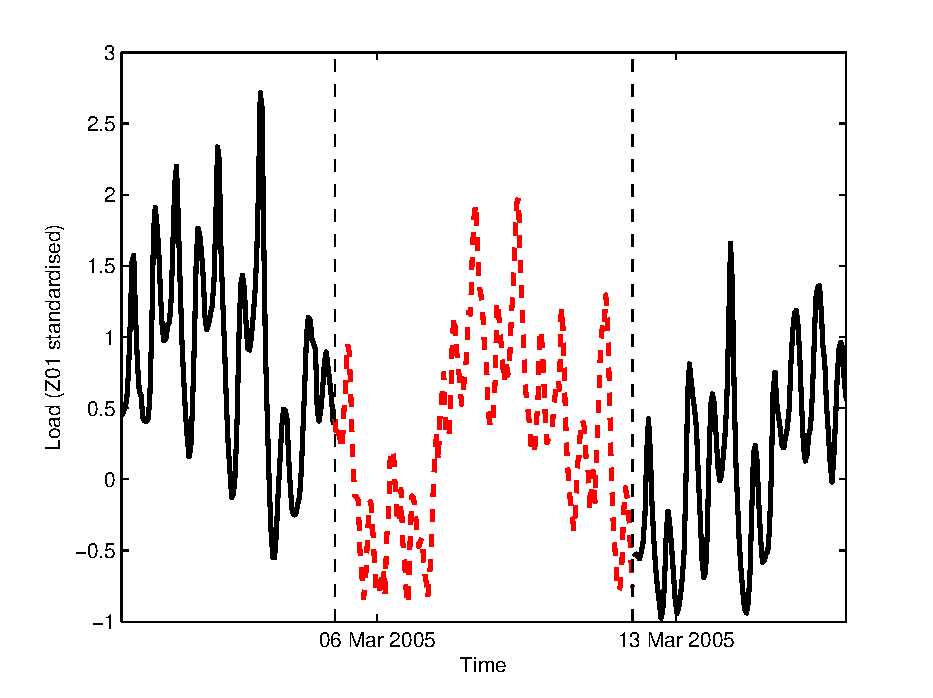
\includegraphics[width=9.0cm]{figures/gefcom/load_pred.pdf}
      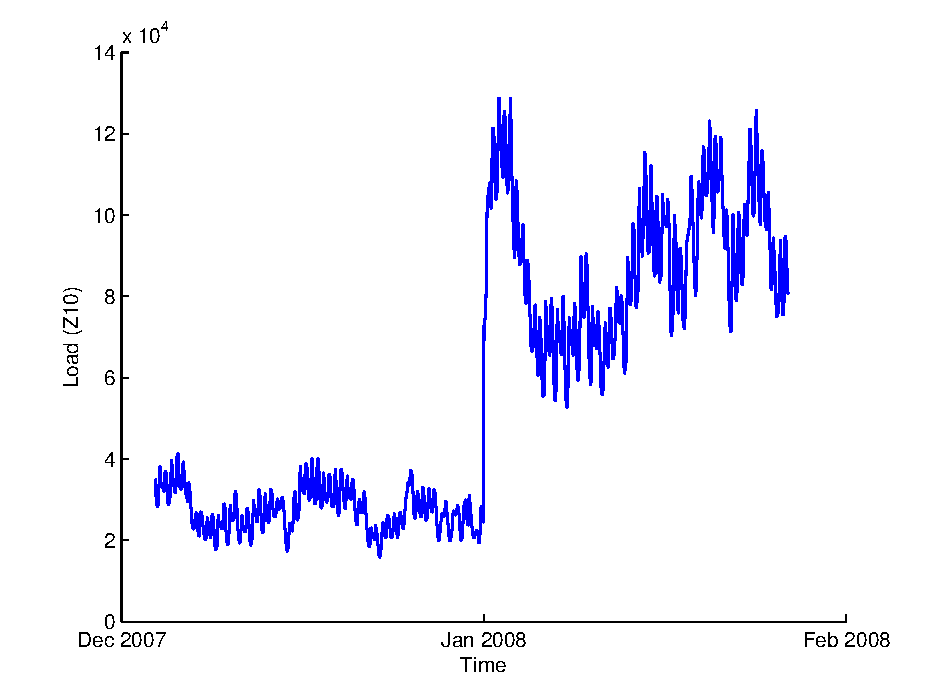
\includegraphics[width=7.0cm]{figures/gefcom/zone_10.pdf}
    };
  \end{scope}
  \begin{scope}[xshift=7.0cm]
    \node [mybox] (box){
      %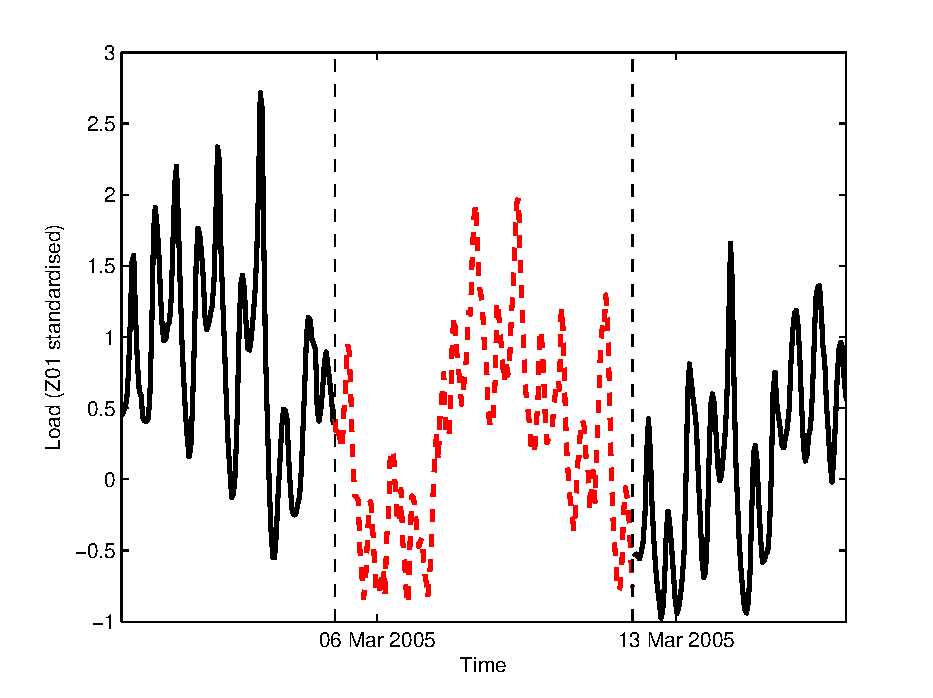
\includegraphics[width=9.0cm]{figures/gefcom/load_pred.pdf}
      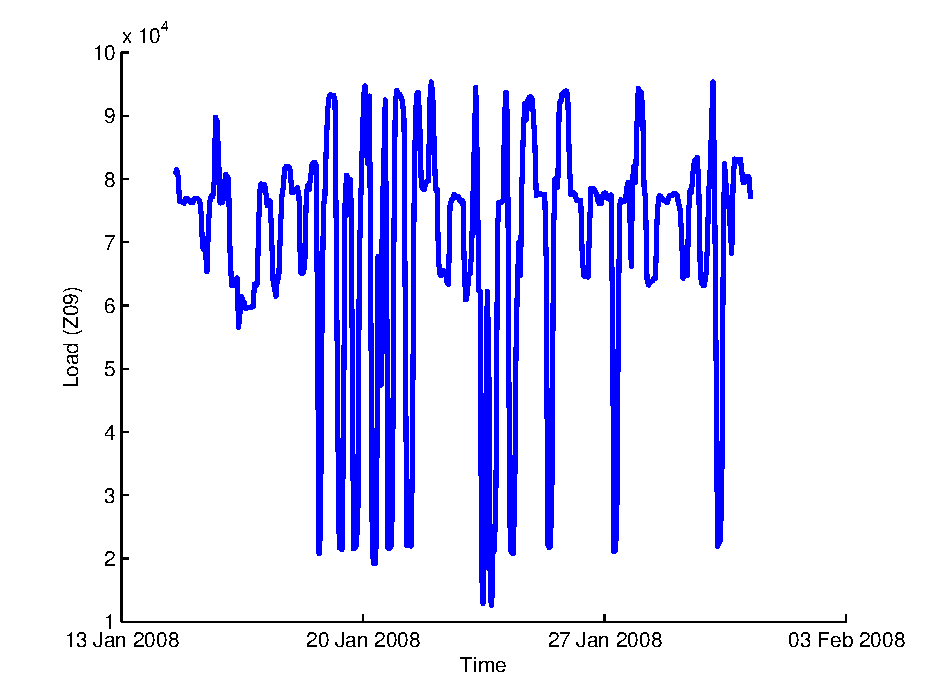
\includegraphics[width=7.0cm]{figures/gefcom/zone_09.pdf}
    };
  \end{scope}
\end{tikzpicture}

  \end{center}
  \caption{Left: Raw data at zone 10, showing a large discontinuity. Right: Raw data at zone 9, showing atypical load dynamics.}
  \label{fig:load}
\end{figure}

This visual analysis revealed a large discontinuity in load series 10 and atypical dynamics in series 9 (see figure~\ref{fig:load} and others for comparison).
No other large anomalies were detected during the first inspection of the data and smaller irregularities were not revisited since the algorithms detailed below performed acceptably well without further data cleansing.

No adjustments were made for holidays or other irregular events such as electricity black-outs.
Ignoring them was merely a practicality of time constraints rather than a design choice.

\section{Temperature forecasting}

\label{sec:temp}

\subsection{Initial analysis and remarks}

The error metric used in GEFCom2012 was heavily weighted towards times at which temperatures were unknown (\ie the load forecast rather than backcasts).
Consequently, good temperature predictions seemed crucial for overall success.

When submitting a solution to Kaggle, the error metric was computed on 25\% of the held out data and returned to the user.
This allowed a user to optimise temperature predictions by optimising the score of resulting load predicitions (\ie computing load predictions based on different temperature predictions and selecting the temperature prediction with the highest corresponding load prediction score).
Depending on how the test data was split (into the 25\% test and 75\% validation partition) this may have allowed users to come very close to knowing the true future temperatures.

\begin{figure}[ht]
  \begin{center}
    \begin{tikzpicture}
  \begin{scope}[xshift=0cm]
    \node [mybox] (box){
      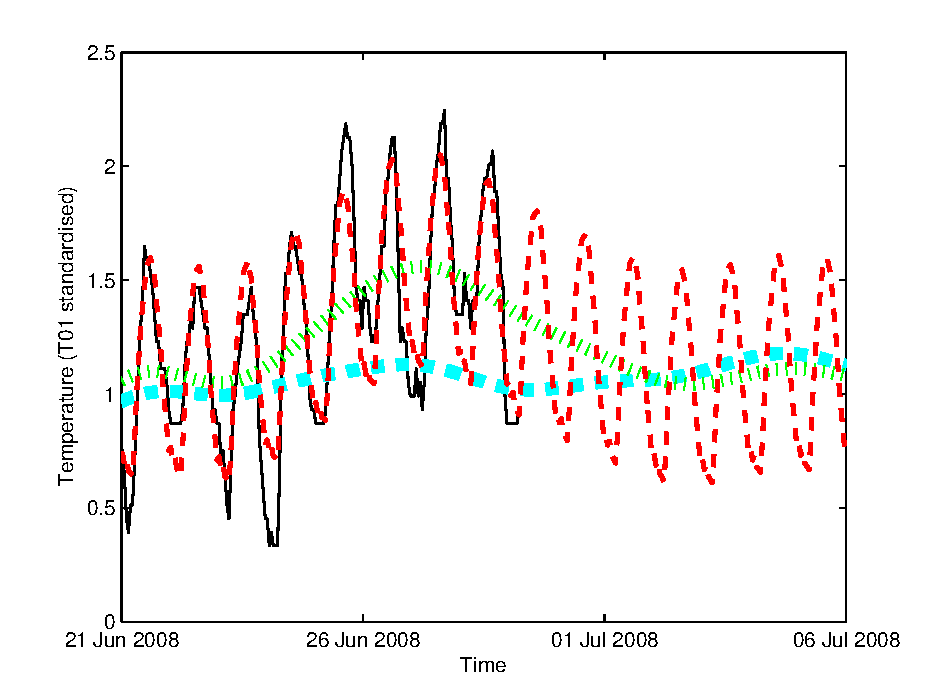
\includegraphics[width=12cm]{figures/gefcom/temp_pred.pdf}
    };
  \end{scope}
\end{tikzpicture}

  \end{center}
  \caption{Raw data at temperature station 1 (after removing mean and scaling to have unit standard deviation) (black solid). Historic average of smoothed temperatures (blue dashed thick). Current and predicted smoothed temperatures (green dotted thick) and final temperature predictions (red dashed).}
  \label{fig:temp_pred}
\end{figure}

I therefore used a flexible but simple method for forecasting temperatures that could be easily tuned.
Figure~\ref{fig:temp_pred} shows data from temperature station 1 along with various curves used for prediction (described later).
The black solid line is the raw data, which shows that temperatures follow a smooth trend with a daily pattern of rising and falling temperatures.
For simplicity, I modelled the smooth trend and daily periodicity separately and modelled each temperature station in isolation.

\subsection{Methodology}

The smooth trend was estimated within the data using local linear regression \citep[e.g. chapter 6 of][]{Hastie2009-hj} with a bandwidth of one day; see section~\ref{sec:gefcom:auto} for a discussion of how this method could have been usefully replaced by Gaussian process regression.
I assumed that the smooth temperature trend would, on average, smoothly return to the historical average.
A suitable modelling technique that would give this type of prediction is Gaussian process regression; the difference between the smoothed temperature and its historical average was regressed against time using a kernel of the form $\kSE + \kWN$ \ie a smooth function plus noise.

In Figure~\ref{fig:temp_pred}, the thick blue dashed curve shows the historical average of smoothed temperatures and the thick green dotted line shows the current smoothed temperature and prediction.
The parameters of the GP model (length scale and scale factor of the squared exponential kernel) were tuned by hand, initially choosing sensible values based on plots of the data and then trying to optimise the public test score of derived load predictions.

The difference between the temperature and the smoothed temperature was assumed to be a smooth periodic function with a period of one day.
This modelling assumption was implemented using a Gaussian process with a periodic kernel (again regressing the difference against time).
Parameters of the GP model were chosen by optimising the marginal likelihood of the model given particular parameters using optimisation methods supplied in the GPML toolbox\footnotemark.
Only the last 250 data points (which corresponds to approximately 10 days) were used to fit this part of the model in order to capture recent temperature dynamics.
\footnotetext{\url{http://www.gaussianprocess.org/gpml/code/matlab/doc/}}

\subsection{Replication of results}

The spreadsheet and scripts used to manipulate the temperature data can be found in the folder \texttt{temp}.
The MATLAB script makes use of the GPML toolbox which is contained in the folder \texttt{GPML}.
The temperature data was reshaped into a (time) $\times$ (temperature station) array using the spreadsheet \texttt{temp.xlsx} and then saved in \texttt{times\_series\_raw.csv}.
The method described above is implemented by the MATLAB script \texttt{predict\_temp.m} which saves the predicted time series in \texttt{GP\_pred\_temp.csv} and the smoothing of these predictions in \texttt{smooth\_temp\_GP.mat} and \texttt{smooth\_temp\_GP.csv}.

\subsection{Discussion}

The red curve in Figure~\ref{fig:temp_pred} shows the result of the methodology applied to temperature station 1.
The fit to the data is far from perfect but it has captured the broad features of the data.
Given the time constraints of this competition I did not investigate the temperature / weather forecasting literature; far better methods must certainly exist!

\section{Gradient boosting machines}

\label{sec:gbm}

\subsection{Initial analysis and remarks}

\label{sec:gbm_init_anal}

\begin{figure}[ht]
  \begin{center}
    \begin{tikzpicture}
  \begin{scope}[xshift=0cm]
    \node [mybox] (box){
      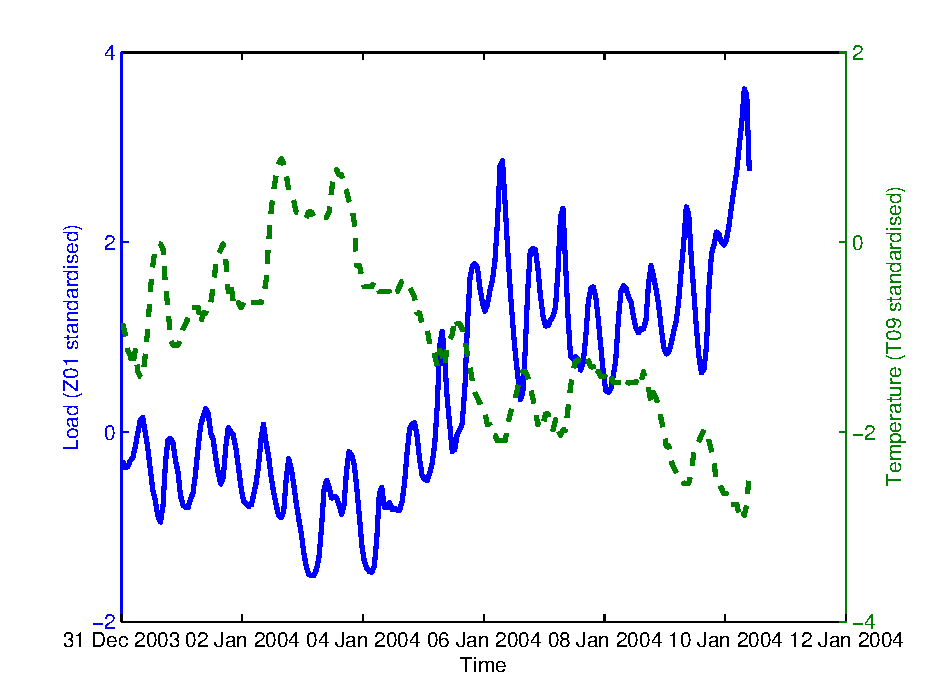
\includegraphics[width=12cm]{figures/gefcom/gef_load_z01_t09_250.pdf}
    };
  \end{scope}
\end{tikzpicture}

  \end{center}
  \caption{Raw data at load zone 1 (after removing mean and scaling to have unit standard deviation) (blue solid) and raw data at temperature station 9 (after removing mean and scaling to have unit standard deviation) (green dashed).}
  \label{fig:load_temp}
\end{figure}

Figure~\ref{fig:load_temp} plots a subset of the data for loads at zone 1 and temperature station 9.
We can see that that the load has a smoothly varying trend with roughly periodic daily deviations from this trend.
The load also appears to be negatively correlated with temperature in this region of data.
It is also reasonable to assume that load dynamics will be different on weekends compared to weekdays.

Based on these observations, I modelled loads as a function of time of day, time within week, temperatures and smoothed temperatures (all stations).
All zones were modelled independently for simplicity.

\subsection{Methodology}

A standard `black-box' technique for learning an unknown regression function is that of using gradient boosting machines (GBM) \citep[e.g. chapter 10 of][]{Hastie2009-hj}.
For each zone I used all of the data to train a GBM and then used that to predict all outputs \ie I learnt a global function for each zone.

I used a standard R implementation of GBM using most of the default settings\footnotemark.
After some brief experimentation with parameter values I used a shrinkage factor of 0.01, 10000 trees and an interaction depth of 3.
I experimented with other parameter values, using the public test score as a guide, but nothing I tried improved upon my initial guess and therefore I did not expend much effort trying to optimise parameter values.

\footnotetext{\url{http://cran.r-project.org/web/packages/gbm/index.html}}

\subsection{Replication of results}

The scripts and data used can be found in the folder \texttt{gbm}.
The load data was reshaped into a (time) $\times$ (load zone) array using the spreadsheet \texttt{load.xlsx} in the folder \texttt{load}.
This was then concatenated with the temperature predictions and smoothed temperature predictions and saved in \texttt{gbm\_input.csv}.
The R script \texttt{basic\_gbm.R} then performs the method described above to produce predictions which are saved in \texttt{gbm\_output.csv}.

\subsection{Discussion}

The time series for zone 10 had a very large discontinuity (see left of figure~\ref{fig:load}).
GBM was used as a global prediction method which means it will have produced very bad predictions for zone 10.
I later fixed this by modelling the loads either side of the discontinuity separately.
Perversely, this resulted in a worse public test score.
However, this change resulted in a much improved private test score; in hindsight I should have opted for the more reasonable model!

\section{Gaussian processes}

\label{sec:gp}

\subsection{Initial analysis and remarks}

The observations made about the load data in section~\ref{sec:gbm_init_anal} (\ie smooth trends, near periodic variations, dependence on temperature) can be modelled using Gaussian process regression.
As demonstrated in chapter~\ref{ch:construction} specifying the kernel function of a Gaussian process allows one to encode these structural assumptions into a regression model.

\subsection{Methodology}

Three different kernel functions were used; one for backcasting, one for forecasting and one for backcasting zone 9.
The forms of the three kernels used were as follows\footnotemark
\footnotetext{See source code for parameter values}
\[
& \kSE_t + \kSE_S + \kSE_t \times \kSE_T \times \kPer_t \label{eqn:kernel1}\\
& \kSE_t + \kSE_t + \kPer_t \label{eqn:kernel2}\\
& \kSE_t + \kSE_S + \kSE_T \times \kPer_t \label{eqn:kernel3}
\]
where the subscripts indicate which dimension the kernel acts upon; (t)ime, (T)emperature or (S)moothed temperature.
For backcasting, the model was applied to the 1000 surrounding data points; for forecasting the last 500 data points were used.
Only one temperature station was used in this method; for each back / forecasting region the model evidence of the model was computed for each temperature station.
Bayesian model averaging \citep[e.g.][]{Hoeting1999-tn} was then used to combine the predictions.
In practice this was usually numerically equivalent to selecting the model / temperature station with the highest model evidence.

Kernel~\eqref{eqn:kernel1} encodes the assumptions that loads can be explained as a smoothly varying trend and an approximately periodic component.
The smooth trend is the sum of a smooth function of smoothed temperature and a smooth function of time (to explain any deviations from the trend implied by temperature).
The periodic component can vary through time and by being multiplied by $\SE_t$ and $\SE_T$ the shape of the periodicity will be more similar to recent times and any points in time with similar temperatures.
This kernel was used for backcasting all zones apart from zone 9.
An example of this kernel in action is shown in Figure~\ref{fig:load_pred}.
The left plot shows the load data (black solid) and the prediction (red dashed).
On the right is the temperature time series which resulted in the model with the highest model evidence.
Comparing the two plots we can see that the deviations of the prediction from the trend through time correspond to fluctuations in the temperature time series.

\begin{figure}[ht]
  \begin{center}
    \begin{tikzpicture}
  \begin{scope}[xshift=0cm]
    \node [mybox] (box){
      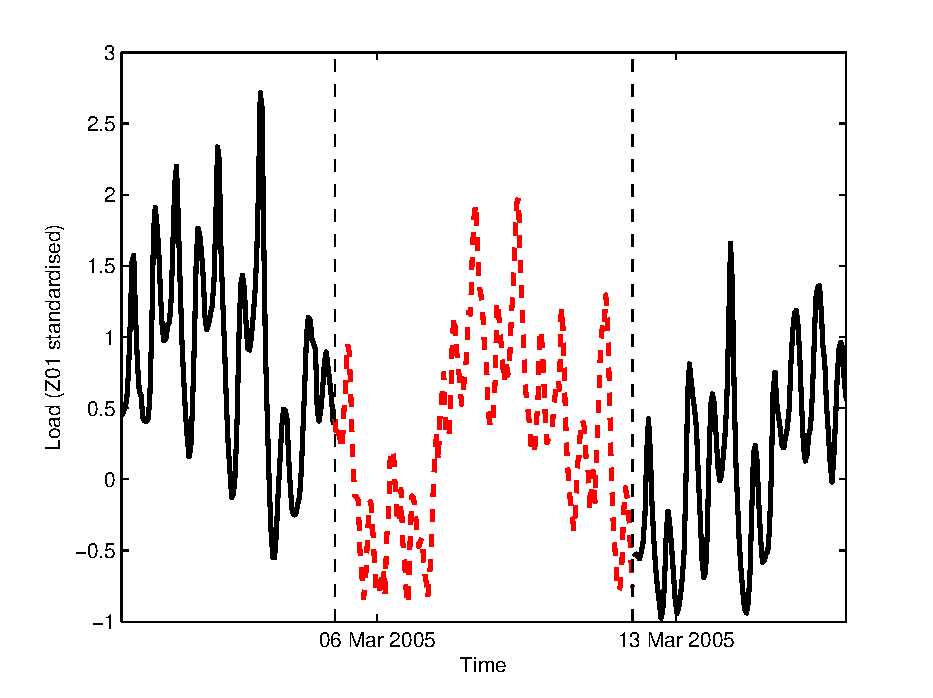
\includegraphics[width=7.0cm]{figures/gefcom/load_pred.pdf}
    };
  \end{scope}
  \begin{scope}[xshift=7.0cm]
    \node [mybox] (box){
      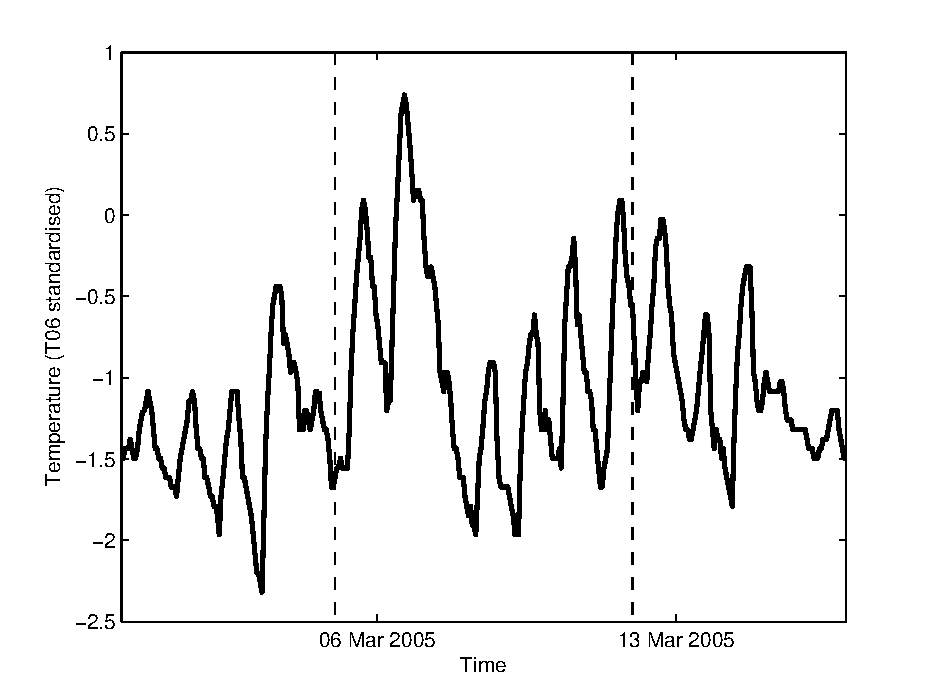
\includegraphics[width=7.0cm]{figures/gefcom/best_temp.pdf}
    };
  \end{scope}
\end{tikzpicture}

  \end{center}
  \caption{Left: Raw data (after scaling and translation) (black solid) and Gaussian process predictions (red dashed) for zone 1. Right: Corresponding temperature time series used for prediction. Notice that the peak in temperature corresponds to a trough in the load predictions \ie the model has predicted a negative correlation between temperatures and loads.}
  \label{fig:load_pred}
\end{figure}

Kernel~\eqref{eqn:kernel2} encodes the assumption that loads can be explained as the sum of two smooth functions with different length scales and an exactly periodic smooth function.
This simpler kernel was used for forecasting since it gave more stable extrapolations of the data.

Kernel~\eqref{eqn:kernel3} is a simpler version of kernel~\eqref{eqn:kernel1} used for backcasting zone 9.
The periodic component is now only similar to other times with similar temperatures.
This prevented the predictions from being so greatly affected by the large isolated load fluctuations present in zone 9.

The forms and parameters of the kernel functions (see the accompanying code for all of the values) were chosen by trial and error (observing which kernels gave reasonable looking predictions and computing public test scores).

\subsection{Replication of results}

The spreadsheet and scripts used can be found in the folder \texttt{gp}.
The load data was reshaped into a (time) $\times$ (load zone) array using the spreadsheet \texttt{load.xlsx} in the folder \texttt{load} and then saved in \texttt{load\_input.csv} which encodes missing values as zeros.
The outputs of the temperature prediction \texttt{GP\_pred\_temp.csv} and \texttt{smooth\_temp\_GP.mat} are used directly.

The MATLAB script \texttt{gp\_elec.m} performs the methodology described above, saving the predictions to \texttt{gp\_pred.csv}.

\subsection{Discussion}

Selecting the form and parameters of the kernels by hand required a moderate amount of familiarity with Gaussian processes.
It is likely that better performance could have been achieved by the larger and more principled search over kernel functions introduced in chapter~\ref{ch:construction}.
Barriers to its immediate application are however discussed in section~\ref{sec:gefcom:auto}.

\section{Selecting the final ensemble}

\label{sec:ensemble}

\subsection{Remarks}

The final prediction was formed as the ensemble (weighted average) of predictions from three separate methods; gradient boosting machines, Gaussian process regression and the benchmark solution provided by the competition organisers (a linear model).
Ensembling is a very powerful technique for combining predictions from separate models.
If two predictions (viewed as random quantities) are statistically uncorrelated then their average will have lower variance than either one separately.

In practice, different algorithms are correlated and ensembling highly correlated predictions will rarely lead to improved performance.
In particular, I also tried the random forest algorithm\fTBD{ref} but the predictions were too correlated with gradient boosting machines (they are both based on an ensemble of decision trees) to be a useful addition to the ensemble.

\subsection{Methodology}

The ensemble weights were chosen by hand, using the public test score as the metric to be optimised.
The public test scores did not vary considerably once sensible parameters had been found so more advanced techniques were not used to optimise the ensemble weights.

\subsection{Replication of results}

The spreadsheets used to manipulate model output can be found in the folder \texttt{ensemble}.
The spreadsheet \texttt{sub\_creator.xlsx} was used to convert (time) $\times$ (load zone) arrays of model output into the required format for submission.
The output of this spreadsheet was then copied in \texttt{ensemble\_creator.xlsx} which performs the averaging to produce ensembles of the predictions.

\subsection{Discussion}

This method could have been been slightly improved by programmatically selecting the ensemble weights, optimising some form of validation metric.
One could also have tried to optimise the public test score directly.
Since only 2 submissions could be tested per day, one would want to use an optimisation technique that made very efficient use of data \citep[e.g.][]{Osborne2009-ti, Snoek2012-ri}.

Larger improvements could likely be achieved by considering a larger number of base predictions.
It is likely that the algorithms used by other competitors in GEFCom2012 would provide useful additions to the ensemble of predictions.
See \cite{Hong2014-yf} and the references therein for an overview of the methods used by other participants.

\section{An attempt to construct the composite kernels automatically}
\label{sec:gefcom:auto}

My participation in this data mining competition provided excellent experience before working on the research described in chapter~\ref{ch:construction} and \cite{Duvenaud2013-dn}.
A natural question to ask is whether or not the compositional kernel search could have been directly applied to this competition, potentially speeding up my development of models and improving performance.
The answer to this question is `mostly' and reveals some interesting shortcomings in state of the art methods of approximate inference for Gaussian processes.
We now present a detailed analysis of the temperature data.
These comments apply similarly to the load data.

The function used to forecast temperatures displayed in figure~\ref{fig:temp_pred} can be described as
\[
  & \textrm{ Average historical smoothed temperatures} \\
  + & \textrm{ A smooth function } \\
  + & \textrm{ A daily periodic function}
\]
which could alternatively be described as
\[
  & \textrm{ An annual periodic function} \\
  + & \textrm{ A smooth function } \\
  + & \textrm{ A daily periodic function}
\]
which could be modelled by a Gaussian process with kernel $\kPer + \kSE + \kPer$ with appropriate parameters.

Exact inference for Gaussian processes has $\mathcal{O}(N^3)$  computational complexity where $N$ is the number of data points.
This makes it (currently) prohibitive to perform exact inference for $N$ much larger than 1000.
The complete GEFCom dataset contained roughly 40,000 data points meaning that one has to consider approximate inference schemes.

A simple approximate inference scheme is simply to use a subset of the data \citep[e.g.][]{Quinonero-Candela2005-er}.
Running the kernel search procedure on a randomly selected 500 data point subset of the data for temperature station 1 results in \TBD{Some stuff - ideally with pictures and descriptions produced automatically}.
While this has captured long term trends and the annual periodicity it has failed to pick up on the daily periodicity.
This is because when subsetting so harshly the daily periodicity is all but invisible in the data (or rather there is insufficient evidence in the data for such a complicated function).

Presented with this failure one might consider instead using a contiguous subset closest to the times at which prediction will be performed.
The results of performing this analysis are \TBD{Some stuff}.
This automatically constructed model now picks up on the daily periodicity but since it only has access to less than 21 days of data there is no way for it to infer the annual periodicity.
There is also insufficient data to infer that whilst the shape of periodicity changes smoothly over time there is a historical average that it should return to.

A potential compromise solution would be to use a subset of data which was a mixture of the two methods already described.
Using this data subset results in \TBD{stuff - probably going to not notice the annual average periodicity}.

There are myriad methods for performing approximate inference in Gaussian processes, but almost all of them either exploit the fact that long lengthscale components do not require much data to learn effectively and short lengthscale components have approximate statistical independence relationships that allow for approximate inference methods.
The above example demonstrates that approximate inference methods may need to deal with these two types of structures simultaneously.

In this particular example a full description of the data might be
\[
  & \textrm{ An annual periodic function} \\
  + & \textrm{ A long term smooth function } \\
  + & \textrm{ Shorter term smooth functions } \\
  + & \textrm{ A daily approximately periodic function} \\
  + & \textrm{ A daily periodic function which is similar to previous values in previous years}
\]
The last term could be modelled with a Gaussian process using a kernel of the form $\kSE \kerntimes \kPer \kerntimes \kPer$.
The most effective subset of data, or more generally type of approximation scheme, is different for all of these different functions.
The annual periodicity and long term smooth function can be learned with a random subset of the data.
The shorter term smooth functions and approximate daily periodicity will require more data to be learned effectively but one will eventually be able to make use of approximate statistical independence relationships between far away data points to learn the function at any point using local data.
For the final function, to learn the function at any point one only needs to see data nearby in time and the corresponding time points in previous years.

One could imagine a type of backfitting algorithm that can exploit the appropriate way to perform approximate inference most effectively for each component function, but perhaps there are methods that avoid the potentially costly iterations of back fitting and also provide estimates of marginal likelihood.
\TBD{Maybe give an example on this data}

\section{Conclusion}

\NA{Rewrite in the light of additional experiments}

In this competition I applied general purpose machine learning / regression algorithms and made few adjustments for the specific domain the data arose from.
Despite this, the resulting predictions were highly competitive.
It is hoped that this report shows that simple techniques can be very effective for predictive modelling and can inspire practical techniques for load forecasting.

\outbpdocument{
\bibliographystyle{plainnat}
\bibliography{references}
}
